\documentclass[12pt, Arial]{article}   	
\title{Teaching a Class to Grade Itself using Game Theory}
\author{Nick Kaashoek and William Wu}
\date{\today}
\usepackage[margin=1in]{geometry}
\usepackage{parskip}
\usepackage{cite}
\usepackage{graphicx}
\usepackage{amsthm}
\usepackage{wrapfig}
\usepackage[section]{placeins}
\usepackage{enumitem}
\setlength{\parindent}{15pt}
\newtheorem{theorem}{Theorem}
\newtheorem{definition}{Definition}
\begin{document}
\maketitle
\section{Introduction}
Over the past few years, there has been a tremendous increase in the popularity of MOOCs (Massive Open Online Courses), as well the importance of MOOCs to education as a whole. Popular MOOC systems such as Coursera or EdX are well funded, which explains their rapid growth: 60 million dollars were invested in EdX when it started in May of 2012~\cite{canmoocsreducecc}. However, the MOOC's main importance comes from its scalability. MOOCs are able to educate massive numbers of students from anywhere in the world~\cite{makingsenseofmoocs}: By the end of 2012, 1.7 million students had attended a course through Coursera~\cite{swotanalysisofmoocs}. The sheer number of students leads to high student-professor ratios that can reach 150,000:1 in some courses.

High student-professor ratios lead to problems for professors. Professors are simply unable to grade hundreds of thousands of submissions. Currently, two types of solutions are used to remedy the problem: automated grading and peer grading. Automated grading relies on machines to grade assignments. However, machines can only check certain types of answers (i.e. multiple choice), severely limiting the depth of the questions asked~\cite{rightandwrongmoocs}. Even though automated grading for written essays is an active area of research with much recent progress, a usable solution does not yet exist~\cite{automatedsystemssuck}. On the other hand, peer grading can grade any type of question, but a system utilizing it could easily be ``hacked'' by the students~\cite{makingsenseofmoocs}. Although both of these systems are interesting concepts, they are limiting or inaccurate in practice~\cite{howaccurateispeergrading}.

The problem of grading large numbers of submissions is important to solve. Without a solid solution, MOOCs cannot provide efficient feedback for their students, rendering them unable to effectively evaluate their knowledge. Because this limits their learning abilities, it is imperative to create an efficient system that enables students to receive feedback to learn efficiently.

There have been many attempts at solving such an important problem~\cite{autograding}~\cite{edxsoftware}. However, this work introduces what previous attempts lack: a rigorous mathematical analysis of the system using tools from game theory and mechanism design. This work sets a concrete set of constraints that a grading system must satisfy to mitigate students' incentive to cheat, as well as a concrete benchmark to analyze the efficiency of various systems. Together, these create a concrete measure for evaluating peer grading systems in terms of efficiency (how much time the professor and students spend grading) and fairness for the students (how accurate their final scores are). Having this measurement model is a large contribution in itself, because it allows comparison between different systems. Although a theoretical model cannot predict exactly what will happen in practice, game theory and mechanism design have a history of generally determining mechanisms that work in practice from ones that do not~\cite{AGTbook}. Mechanisms that do not follow game theoretic constraints may work in the short-term, but they will be exploited if possible in the long term~\cite{boycottfinal}.
%[Note from Matt and Christos: 1) mention that coming up with a model is itself a big contribution, because now we can compare the quality of two different mechanisms. 2) Mention that certainly theory is not a perfect predictor of what will happen in practice, but that game theory and mechanism design (and all the assumptions used in this work) have a history of ``calling good mechanisms good and bad mechanisms bad''. Also, solutions that do not satisfy game theoretic constraints may work for a while, but in the long run if a system can be exploited, eventually it will be. See here for an interesting example of this: http://www.insidehighered.com/news/2013/02/12/students-boycott-final-challenge-professors-grading-policy-and-get]

Game theory allows the creation of a unified system of assumptions that simulate student behavior in a class. The grading system can be viewed as a ``game'' where the set of ``rules'' are known to everyone and the ``players'' --- the students --- ``play'' the game in order to get the best possible result. Using the assumptions and rules, game theory can predict how students will behave when they ``play''. This way, mechanism efficiency and effectiveness cam be proved, allowing the evaluation of different sets of rules.

The difficulty of the problem lies in finding an incentive for students to spend time to grade assignments of others who they don't care about. Incentivizing students seems simple at first: let the professor give bonus points to students who grade, for example. However, this may not return anything useful because a clever student will just take the points and assign a generic grade (i.e how can the professor tell the difference between an accurately assigned hundred and randomly awarded 100). The next step would be to implement simple checking: e.g. have each paper be graded by two students who both receive bonus points if their grades match. This case may work if the students are isolated, but the professor still can't tell the difference between a randomly or sincerely awarded grade. This way, their papers will match those of other clever students, giving them points without grading. These examples show that properly incentivizing graders can be a difficult task. The main purpose of this work is to devise mechanisms which avoid these problems, allowing for work to be distributed efficiently.

As demonstrated by the above examples, the difficulty of the problem lies in the complex behavior of selfish human beings. Because human nature dictates that people will do whatever is in their best interest and may try to outsmart the system, coming up with a strict set of rules to encourage the desired behavior can be quite challenging. A mechanism should be made as simple as possible, but the above examples show that a small amount of simplicity must be sacrificed to obtain a system that can't be manipulated.

This research opportunity is made interesting by the complexity of human nature as well as its necessity for practical use. This paper will cover the thought process of mechanisms leading up to the final mechanism of grading, as well as explain the final mechanism and its implications. All mechanisms and related calculations will be presented. Section 2 describes the mathematical definition of the problem as well as its rules and assumptions.

\section{Materials and Methods}
\subsection{The Scenario}
In our trying to find a solution to the professor's problem, we consider the case of a single assignment. To apply them to an entire class, simply apply them to each assignment. In such a ``round''of grading, there are $n$ students, who each bring one ungraded paper to the professor. These ungraded papers are like the input for a function. Each of these papers, $i$ has an objective score $o_i\mid 0<o_i<100$. This is the score the professor would give out. Our mechanism then has the students grade the papers in a clever way and output the grades. We identify the students by an index $i$ from $1$ to $n$ and the professor as index $0$.
\subsection{Assumptions}
To create the models that are used to predict the behavior of the students, we use a set process every each time. To begin with, we create a set of assumptions. These assumptions are used to explain how students will act in a given situation; for example, one assumption could be that students want good grades. This is a logical assumption that is likely true, as all the assumptions are, and can be used to classify the behavior of the students in a model. The same set of assumptions can be used for multiple models, which will allow us to evaluate different models side by side. To begin with, a simple set of assumptions was created:
\begin{enumerate}[itemsep=0pt, parsep=0pt]
	\item Students want good grades
 	\item Doing work makes students unhappy
  	\item Students want to be happy
 	\item Students only care about their final happiness
  	\item The happiness of a student is only affected by their grade and the amount of work they do
\end{enumerate}
However, we wanted to create a mathematical solution, so these assumptions need to be changed into math terms. The result of this is as follows:
\begin{enumerate}[itemsep=0pt, parsep=0pt]
  \item Students all share a common happiness function, $H(g)$, where \emph{g} represents the grade the students received, and the output is their happiness. w.l.o.g. $H(0)=0$
  \item Students can grade others' work accurately (i.e they can find $o_i$) but doing so costs one unit of happiness. Therefore after grading $W$ papers, a student's happiness can be expressed as $H(g)-W$
  \item Students want to maximize their final happiness, expressed as $H(g)-W$
  \item Students only care about the expectation of their final happiness, which, put in game theory terms, makes them risk neutral (i.e, if $H(x)=10$ and $H(y)=5$, then getting x and y each with 50 percent chance, gives a happiness of 7.5).
  \item The final happiness depends only on the grade assigned to the student and the amount of effort exercised. It doesn't depend on the score of others
\end{enumerate}

\paragraph{Why?}
There are two questions that need to be addressed, first, why is happiness important, and second, why are the scores of others not important? Happiness is important because it provides a measure of the combination of the work performed and grade received. The reasoning for not caring about friends is due to the relatively low impact they have on someone's grades and happiness, for example, in a coursera course with 150,000 students, it is extremely unlikely that any student will ever be able to have any effect on the grade of another student. So, for simplicity, we ignore the ``friendship''effect.
\subsection{First major objective}
The first goal of the system is to make sure that every student gets the most happiness when they correctly grade every assignment that the professor asks them to. If a system has this property, then it is reasonable to assume that students will always choose to grade every assignment the professor asks them to. Without this property, a system becomes extremely unpredictable. So, in other words, no student can deviate from the truthful strategy to improve his happiness. In math terms, if by acting honestly student i grades $w_i$ papers and gets a grade of $g_i$ there shouldn't be any way for the student to spend $w'_i$ units of effort and get a score $g'_i$ where $H(g'_i)-w'_i > H(g_i)-w_i$.

\subsection{Benchmark}
%Efficiency objective%
The next step is to create a system that will allow multiple different mechanisms to be compared and evaluated side by side; in other words, a benchmark needs to be created. To do this, two things need to be addressed: how accurate the grades the mechanism produces are, and how happy people are. Because happiness can be directly expressed as a function of work, the two things that need to be evaluated are how accurate the grades are, and how much work is being done. As such, the benchmark becomes a sum of the amount of work done by the person doing the most work and the maximum deviation from the correct grades; the lower the sum, the more efficient the mechanism. In mathematical terms we want to minimize the function $max_{i \ge 1} |H(g_i)-H(o_i)| + max_{i \ge 0} w_i$ in the worst possible case.

When creating this benchmark, there are 2 things that need to be considered. First of all, caring about accuracy. This is important because if we don't care, then we could give everyone a 100, which, as explained earlier, is a terrible mechanism. Secondly, caring about work done. If we don't care about the amount of work done, we could have the professor grade everything, which is bad because it makes the professor extremely unhappy. 

Also, we need to address why we use maximum for these two things, and not sum. Caring about the maximum difference in grades and not the sum. Consider these two outcomes: each student's real grade should be 90 but they get a 91 and each student's real grade should be a 90, but all of them get a 90 except for 1 who gets a 0. In this case, the first case is clearly better, something that is only captured by a maximum. To address caring about the maximum work done, consider these two outcomes: one where a professor grades all $n$ papers, and another where each student grades $2$ papers. In this case, the first scenario is far worse, even though the total work performed is less than the second. For this reason, we use a maximum.



% We now have a well defined problem that we need to solve. Of course the set of assumptions might not be very realistic as we will so we 

Now that a simple set of assumptions and a benchmark have been created, it becomes possible to create simple mechanisms, and improve upon them until we get to a final, satisfactory mechanism.

To improve upon our mechanisms, we need to often change our assumptions. This means that the original set of assumptions we proposed will change throughout the course of the paper to allow mechanisms to handle more complex situations.

One advantage of this is that we can now address the fact that the above set of assumptions is rather simple and unrealistic, for instance assuming that every student is a perfect grader.
%Repeat above corrections%
\section{Results}
Once the rules and assumptions have been defined and the benchmark determined, different grading mechanisms can be created and tested. This is where mechanism design and game theory comes into play. Mechanism design is used to create a system that satisfies a set of constraints and achieves a certain purpose. Then, game theory is used to mathematically predict student behavior to benchmark such a system. Starting from the simplest and most obvious approaches, various mechanisms were created, tested, and refined upon in an iterative process that spanned several months. The end result is fairly complete, although there are still questions to be answered in future work.

\subsection{The Calibration Mechanism}

\subsubsection{Mechanism}
First, we design a mechanism that does extremely well in a model defined by our simple and unrealistic assumptions, which we used as a starting point.
\begin{definition}(Calibration Mechanism)
In this mechanism, the professor chooses one paper to grade, which he gives to every student, along with a second, ungraded paper. If the students fail to grade the paper the professor graded correctly, they get a 0. Otherwise they get the minimum of an arbitrary number $???$ and the grade their assigned grade.
\end{definition}
\begin{theorem}
With this mechanism, all students should behave honestly and the mechanism shoul output accurate grades while maintaining a low amount of per-person work.
\end{theorem}
\begin{proof}[Why this works]
See figure~\ref{fig:calibration} on page~\pageref{fig:calibration}.

G is the maximum of \{ some minimum value, the assigned grade \}.
The happiness of one student grading one paper is equivalent to $\frac{H(G)+H(0)}{2}-1$ Because the students have a 0.5 chance of getting a 0, and a one-half chance of getting G.

If they grade both papers, their happiness will be equal to $H(G)-2$Because they spent two units of energy, and are guaranteed to get G.

If they grade neither then the happiness will be $H(0)$ Because they automatically get a 0, but spend no energy.

This means that if $H(G) - 2 > H(0)$, then student will grade both papers. So, for the professor to guarantee that the students use effort and obtain the correct grades, $H(???) > H(0) + 2$.
The teacher expends one unit of effort, each student spends 2, as long as the teacher set the minimum value high enough.
Everything above $H^{-1}(2)$ will be graded correctly, while everything below it will receive a score of $H^{-1}(2)$.
So, maximum deviation is $H^{-1}(2)$, because this is the score that might be given to someone who deserves a 0. Expressed in happiness units, the value is 2.
\end{proof}
\subsubsection{Benchmark}
The means that the value of the objective function in this case is 4, a very low value, because it is exactly the same as if we convinced every student to grade accurately grade 4 papers.

\subsubsection{Problems}
This mechanism is extremely simple, and relies on the unrealistic assumption that students are unable to communicate with each other. If they were able to, students would be able to figure out which paper is calibrated by checking which one they all share.

\subsection{Improved Calibration Mechanism}
\subsubsection{The Mechanism}
In the calibration mechanism, we assumed that students couldn't communicate with each other. For this mechanism, we relax this assumption, thus changing assumption number 11, which now reads as: \emph{All students are able to communicate with each other}
\begin{definition}(Improved Calibration Mechanism)
In this mechanism, we apply the calibration mechanism on a larger scale. Every student grades the papers of \emph{k} other students. The professor also grades every \emph{kth} paper, these are the calibrated papers. The same system for assigning grades is used as in the calibration mechanism.
\end{definition}
\begin{theorem}
In this mechanism, students will return accurate grades, even though they can communicate with each other.
\end{theorem}
\begin{proof}
In this scheme, because of the overlapping papers, the students have no better way of figuring out which papers are calibrated than random guessing, even though they can all communicate with each other. As such, there are 3 options for the students. They can grade 0 papers, giving them a happiness of $H(0) = 0$ or grade all the papers they are assigned, giving them a happiness of $H(g) - k$ or they can grade $i$ papers giving them a happiness of $\frac{i}{k} \cdot H(G)-i$. This means that it is always worse to grade i, because happiness from grading i is equal to i times happiness for grading 0 plus i-k times happiness for grading k.

Even though the students can communicate with one another, they will have no way to determine which paper is calibrated because there are multiple calibrated papers that overlap, and are thus best off grading all the papers. As long as the minimum value is high enough, the papers will be accurately graded, as before.
\end{proof}
\subsubsection{Benchmark and Problems}
The maximum amount of work will be done by the professor, who has to grade $\frac{n}{k}$ papers, making the benchmark $\frac{n}{k}+4$, a potentially higher value than before. The huge problem with this is the high amount of work being done.

\subsection{The Deduction Mechanism}
With this mechanism, we aim to fix the faults of the previous mechanism while retaining the same set of assumptions. Other than reducing the workload, we aim to accomplish the same goals as the improved calibration mechanism.
\subsubsection{Mechanism}
See figure~\ref{fig:deduction} on page~\pageref{fig:deduction}.
\begin{definition}(Deduction Mechanism)
In this mechanism, each paper is randomly assigned to 2 students. Students deduct as many points as they want, and write a justification for each of them. For each paper graded by students $i$ and $j$, where $i$ took of $x_i$ points and $j$ took off $x_j$, sudent $i$ receives contribution score $\frac{x_i}{x_i + x_j}$, and j receives $\frac{x_j}{x_i + x_j}$. Students may then choose to appeal their paper's grade if they are unhappy with it, at which point the professor grades it and gives an incorrect grader a 0. To compute the final score for a student, their final grade on the assignment is calculated as follows: 4 points times their contribution score are added or subtracted to $H(g)$. (Then the student’s grade is converted from Happiness to an actual score).
\end{definition}
\begin{theorem}
The addition of the contribution score being added or subtraced should encourage graders to honestly grade papers, for fear of losing points and the possible reward.
\end{theorem}
\begin{proof}
The graders have two choices, they can either grade the papers, or not grade them.

If the grader does not grade the paper, what score should he or she give it?

If they take off any points, the points will surely be refuted by the professor during the regrade.
So if they take off any points, they will get a 0 on the grading assignment.
If the grader's give it 100, they might get 50 if the other grader also gives it 100. If he gives it anything else, the original grader will get 0.\\
If the grader does grade the paper, what score should he give it?

If the grader randomly takes off any points, the points will surely be refuted by the professor during the regrade, and the grader will get a 0 on the grading assignment.
If the grader gives it 100, he or she will get a 0 the grading assignment if his or her partner does not give 100. In the case of agreement, both graders get 50 on the grading assignment.\\
If the grader does grade the paper, what score should he or she give it?

If the grader takes off fewer points than the true score of the assignment, he or she is throwing away free points. If the grader deducts too aggressively, there is a risk for him or her to get a 0 because the score could be refuted. 
Therefore, assigning the correct score is the best because it guarantees at least a 50.

Assuming that the student's partner gives the paper a 100, which is the best thing they could do if they don't grade, then
	If they don't grade the paper, they don't use any effort. So the student's happiness will H(the student's grade on the original assignment). Contribution score = 0
	If they do grade, they use 1 unit of effort by default. But, the student's happiness will be H(the student's grade on the original assignment) + 3. Contribution score = 1
	
If the partner gives the paper its true grade:
	If the grader doesn't grade the assignment, they will give it a 100 and so the grader's contribution score is -1. So their happiness is H(their original grade) - 4.
	If the grader does grade the assignment, they and their partner gave the same grades, so they get a contribution score of 0. This means that their happiness is H(their original grade). 
	
Therefore, it is in everyone's best interest to honestly grade the paper.
\end{proof}
\subsection{Final Assumptions}
Now that we have reached a point far into the research, we have a model that accounts for a very realistic world view, however, the deduction mechanism still has some unrealistic parts, primarily the inablitity to deal with students who are incompetent graders. With this in mind, we designed a final set of assumptions that more effectively simulate a realistic world.

\begin{enumerate}[itemsep=0pt, parsep=0pt]
\item When grading, $w_i=0 \oplus w_i=1$
\item For all students, $g_i \neq o_i$
\item Students all share a common happiness function, $H(g)$, where \emph{g} represents the grade the students received, and the output is their happiness. w.l.o.g. $H(0)=0$
\item Students can grade others' work perfectly but doing so costs one unit of happiness. Therefore after grading $W$ papers, a student's happiness can be expressed as $H(g)-W$
\item Final happiness is unaffected by other people, only affected by $g_i$ and $w_i$
\item Doing work costs one unit of happiness, so after grading a paper, a student's happiness can be expressed as $H(g)-W$,W is number of work units used
\item Students only care about the expectation of their final happiness, which, put in game theory terms, makes them risk neutral.
\item For a given student in $N$, that student has contact with all other students in $N$.
\end{enumerate}
% Put simply:
% \begin{enumerate}[itemsep=0pt, parsep=0pt]
% \item Students cannot ``half bake''an assignment
% \item Students can't always get the exact objective score
% \item Students want good grades
% \item Students don't like grading
% \item Students are selfish
% \item Doing work costs 1 unit of effort
% \item Students are risk neutral with respect to happiness
% \item All students can talk to each other
% \end{enumerate}
\newpage
\section{Illustrations}
\begin{figure}[!ht]
	\centering
		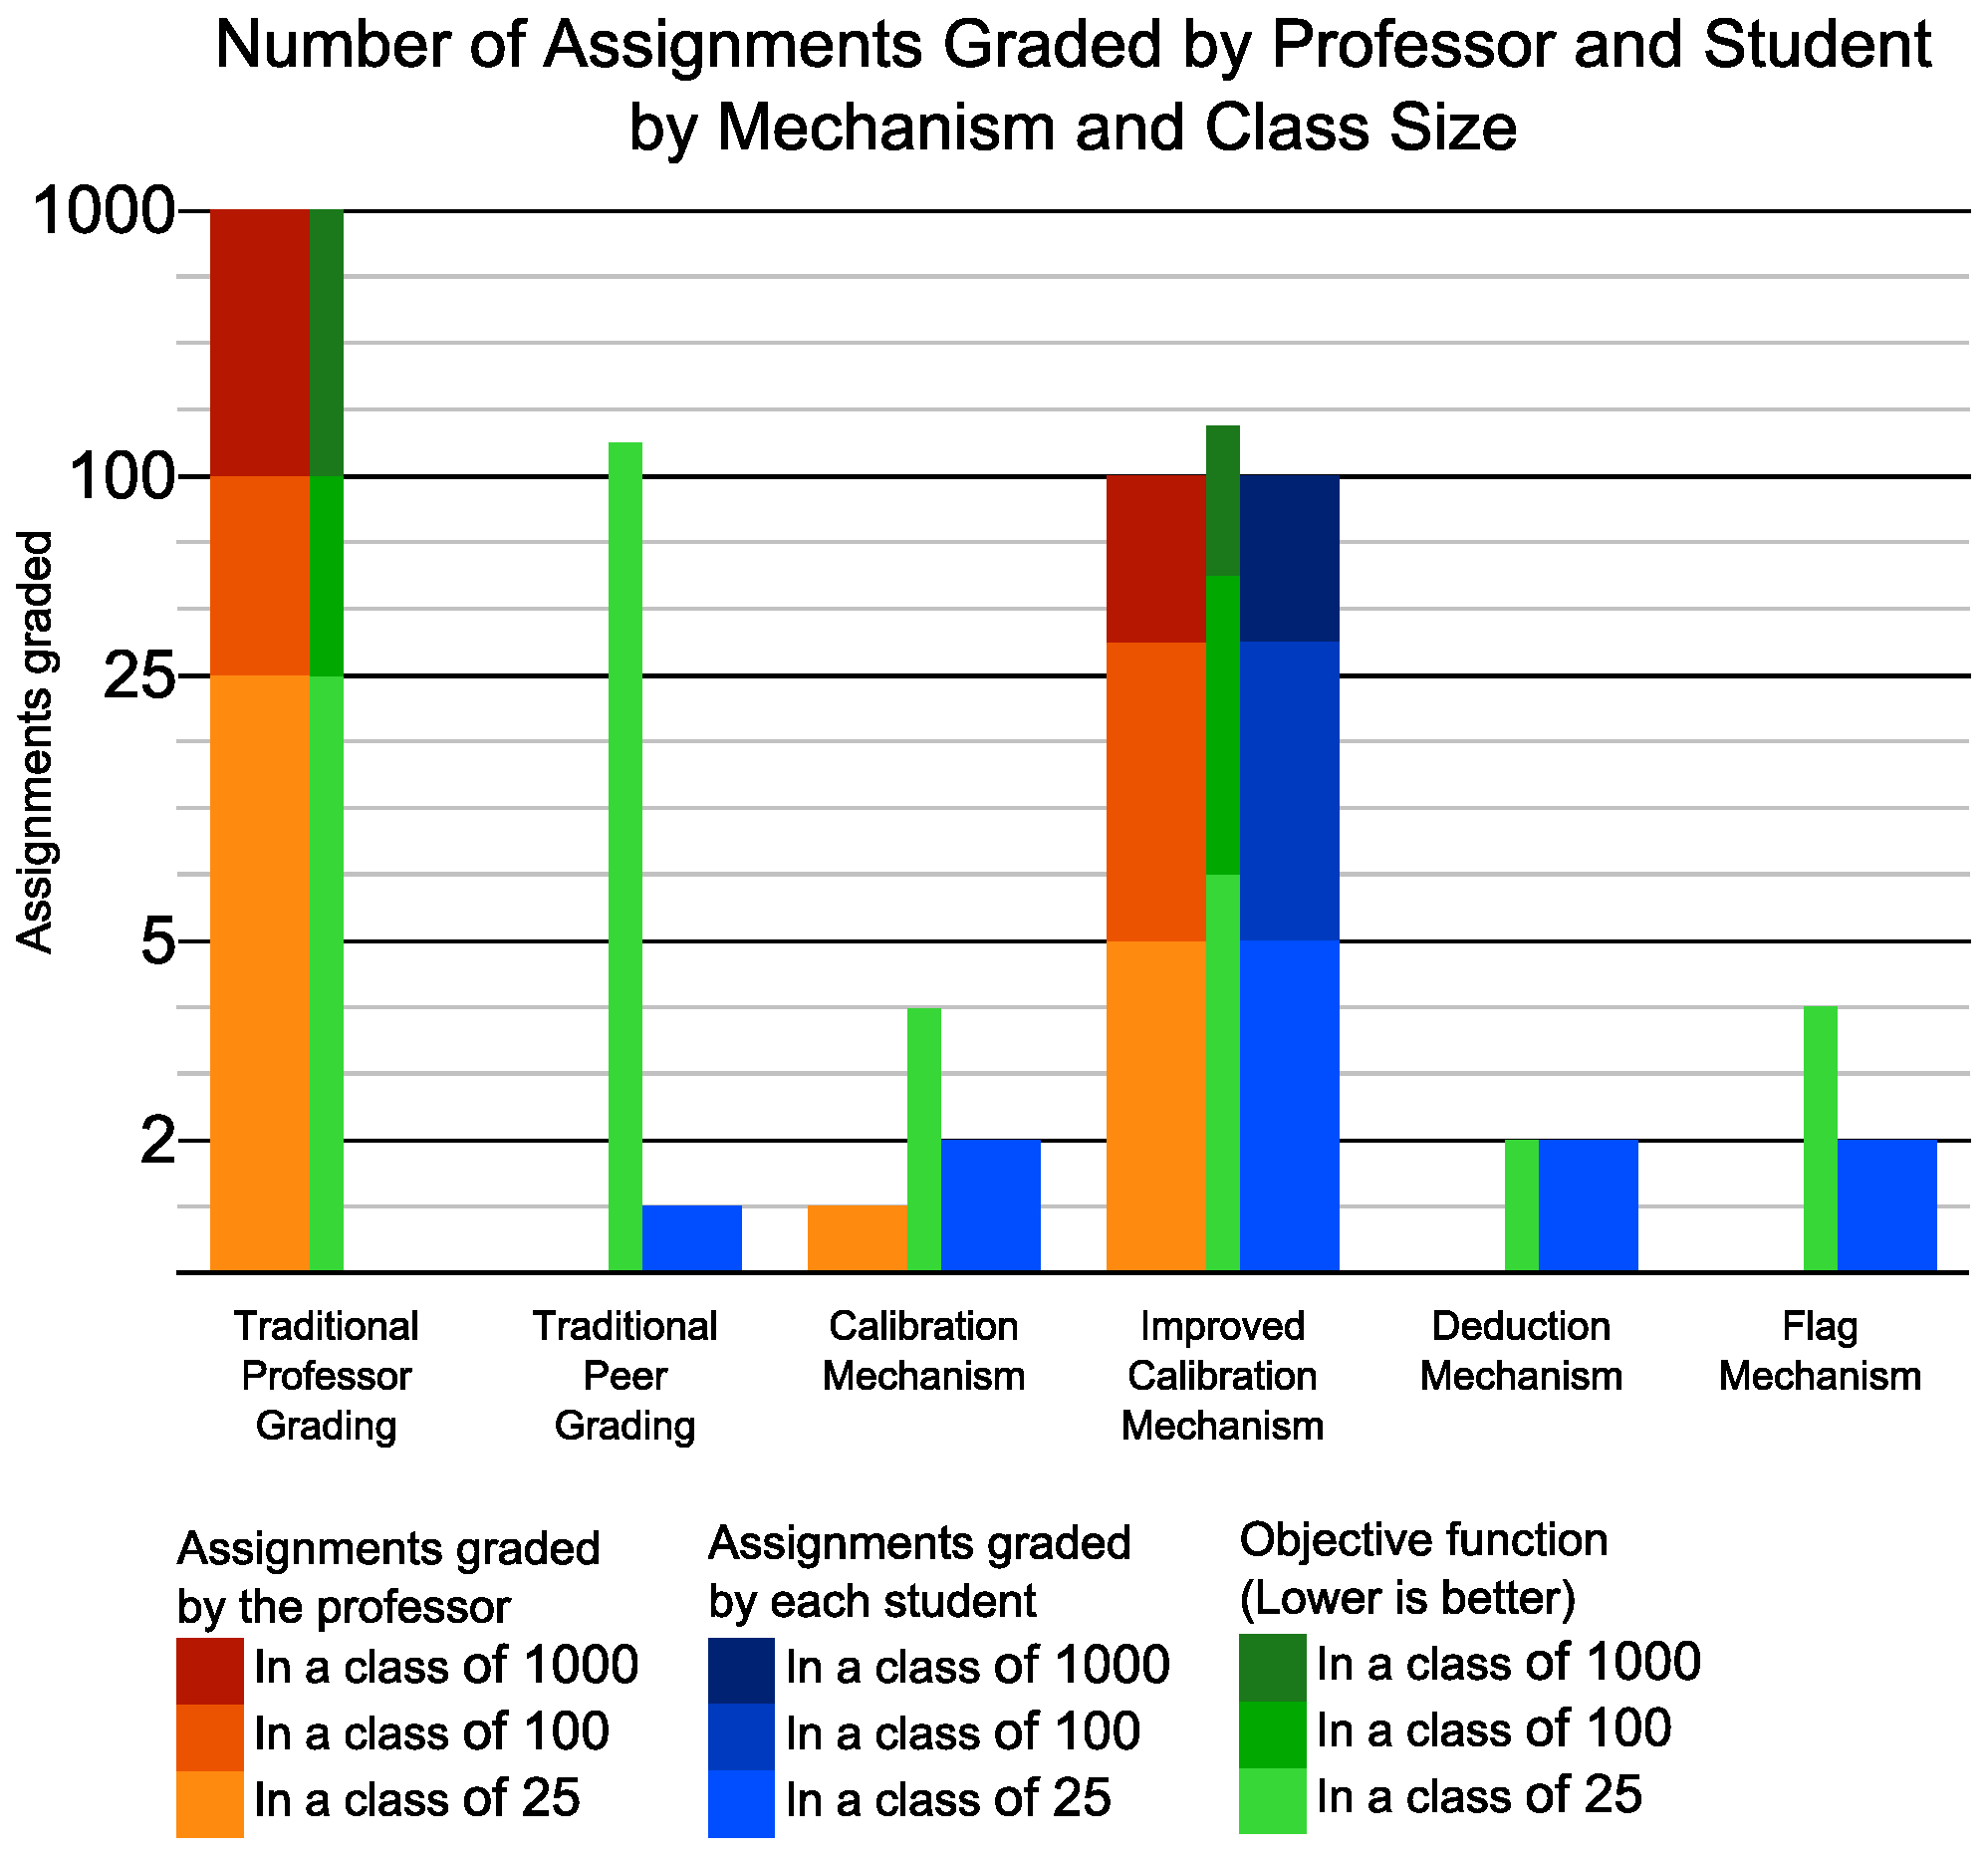
\includegraphics[width=0.9\textwidth]{Comparison.eps}
		\caption {A comparison of mechanisms in terms of scalability, workload, and objective function.}
		\vspace{-100pt}
		\label{fig:Comparisongraph}
\end{figure}
\begin{figure}[!ht]
	\centering
		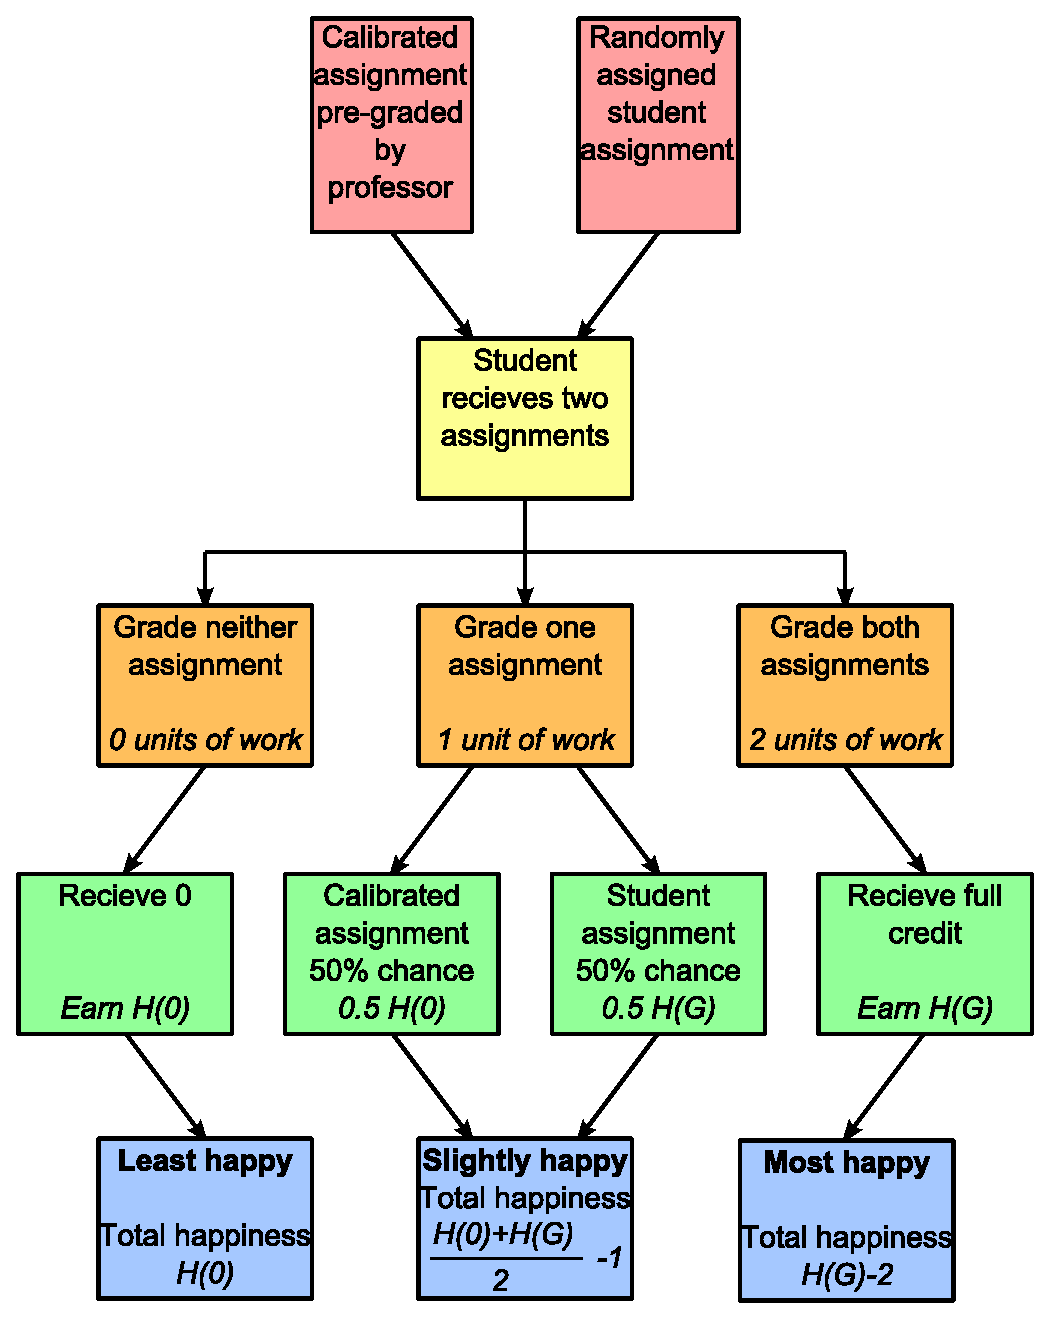
\includegraphics[width=0.75\textwidth]{Flowchart-Calibration.eps}
		\caption {A flowchart of the Calibration Mechanism from the student perspective.}
		\label{fig:calibration}
\end{figure}
\begin{figure}[!ht]
	\centering
		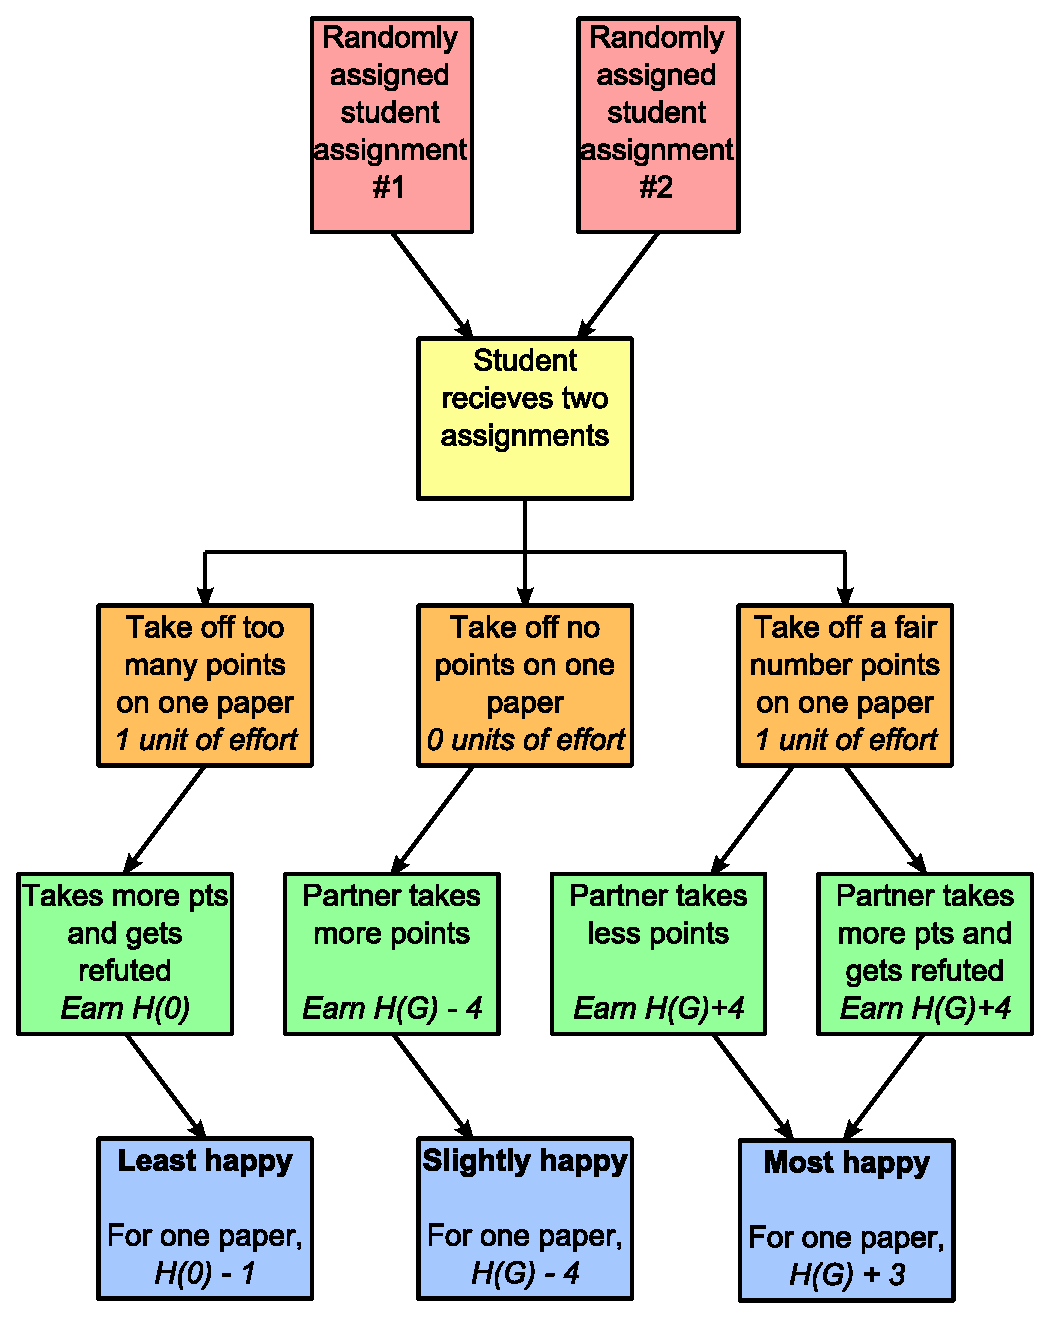
\includegraphics[width=0.75\textwidth]{Flowchart-Deduction.eps}
		\caption {A flowchart of the Deduction Mechanism from the student perspective.}
		\label{fig:deduction}
\end{figure}
\section{Discussion}
With this research, the goal was to create a mechanism that fulfilled our two goals; incentivizing students to play the ``game''the way they were meant to, and to efficiently and effectively grade the assignments of these students. Although our mechanisms are not truly realistic, the significance of them cannot be denied. The mechanisms created by the end of the research came very close to realism, with only one factor missing, and could still be implemented in a classroom environment where all students are capable of grading others assignments efficiently.

The work done in creating these mechanisms further builds upon that which has been done before to try and answer the same question of grading large numbers of papers. Much of the previous work done to address this problem involves creating automated mechanisms that simple spit out machine-assigned grades. These solutions, as stated previously, are inefficient and often produce unsatisfactory results. By creating these mechanisms using game theory, it has been shown that computers do not need to be relied upon to grade papers, opening the way for others to create game theory driven solutions to this problem.

Also, by taking the happiness of the students into account, it can be almost guaranteed that these mechanisms are better for the students than automated grading, or any other solutions attempted before. Many of the complaints that students give out include something along the lines of the fact that they cannot give feedback on their feedback, a problem in the Coursera system~\cite{theproblemswithpeergradingincoursera}. This problem is fixed in our mechanism by allowing the students to appeal their grades and to have multiple rounds of grading. Other commonly expressed problems such as the variability of feedback are also addressed by these mechanisms, which prevent this from happening by having a rigid set of justifications required. This means that students cannot simply pass on a paper with the word ``good,''they must rather take the time to explain why they took off any points they did, or why they gave the paper a perfect score.

Besides making the students happier than they are in other peer grading systems, the mechanisms that result from this research also provide more accurate and legitimate grades for the students. In current peer grading schemes, it is easy for students to just ``game''the system and fake their way through a course. Giving anonymous feedback, for example, does not encourage students to be honest, rather, it gives them a reason to be \emph{dis}honest~\cite{theproblemswithpeergradingincoursera}. This allows students to dishonestly grade the work of others, as well as just give whomever they want a better grade than that person actually deserves. In our mechanisms, however, these problems are solved by removing anonymity and adding incentives to make students behave honestly, no matter who they are grading.

Aside from fixing many problems that students have with other peer grading systems, our mechanisms also address the unhappiness and inconsistency caused by the grading given out by machines. One key problem that machines have is that they always look at the same thing in a paper, meaning that they can be easily ``gamed''and fooled into thinking something is better than it acutely is~\cite{robogradingproblems}. Not only does this make the system inconsistent, but any student who is lacking something that is in the list of requirements the machine checks for can be unfairly given a poor grade, making them unhappy. By solving both of these problems with the mechanisms that were created, it has been demonstrated the peer grading, at least for the moment, is all in all better for education that automated grading.

Not only do the mechanisms developed in this research improve upon the efficiency of automated grading systems, but they also help to remove the dominance that automated grading has placed on grading large courses. By providing a system that fixes many of the problems with current automated grading systems, these mechanisms help to show that automated grading is not the only way to solve the problem of grading online courses. Because automated grading, at the moment, is not as efficient and robust as it needs to be to prevent students from creating unfair situations, this is something that is necessary to show because automated grading is simply not good enough with today's technology.

By creating a mechanism that is, in theory, more efficient than both current peer grading systems and automated grading systems, it has been shown that there is still room for improvement in the grading of online courses. By showing this, a renewed interest in the field can be created, which could lead to others developing more mechanisms that will improve the general education of students in these courses. As the ultimate goal of this research is to accomplish this, the idea that the mechanisms not only accomplish this, but also open the road for others to do so is a marked success.

All in all, with the final mechanism, all of the goals that were set up were accomplished, with only total realism absent from the design. With this final mechanism, it has been shown that it is possible to create a mathematically driven and effective design that can solve a problem that needs to be solved. Not only is this something that has not been done before, but it opens the way for others to build upon this work, something that could eventually lead to the creation of a perfect solution. 

However important the creation of these mechanisms is, arguably more important to the future development of further solutions is the creation of a realistic and robust model. Without a model, many of the mechanisms mentioned would have been impossible to create, and would certainly not work as well as they do. The creation of a model is essential in game theory as it provides the outline for how the ``players''of a given game will act under any set of circumstances. As such, by creating a good model, this research has undergone the trouble of providing a way for anyone to predict how students will behave. 

Not only did this research lead to the creation of a good model, but it also led to the creation of a benchmark. The creation of a benchmark is important because it allows two or mechanisms to be compared side by side, and it allows theorists to definitively determine which of these mechanisms is superior. With this, it becomes possible to compare the results of this research to the results of others, and also allows future work to be done by others. Not only does a benchmark allow the research done here to be compared to that of others, but it allows two totally independent mechanisms not derived from this research to be compared, which could lead to a universal system of evaluating peer grading systems.

Both of these are major contributions towards further developments in the field of research this problem takes place in, primarily game theory. By doing so, grading mechanisms across online courses will constantly be able to evolve and improve with contributions from anyone. By creating the benchmark and model, all mechanisms will undergo a uniform set of evaluations that will allow online course systems to determine which system is the best out of any proposals. By doing so, this research has opened up a road for many game theorists to develop and analyze new ideas that will lead to improvements in student happiness and results from online courses.

Due to the numerous possibilities the creation of a model and benchmark can lead to for future research, it is clear that they are the most important results gained from this research. Without them, nothing else could have been done, and no future mechanisms could be created that would be able to be analyzed in the same way that these were. Due to the importance of future research in this field, it was imperative that this research led to more solutions in the future, so that the problem that was identified would be quickly and efficiently solved.

Although the models presented by this research are not completely realistic, they do show that there is much room for improvement in the area of grading online courses, and that it is possible to take a strictly mathematical approach at designing a mechanism, and then implementing it using computer science. By showing that this is possible, a huge amount of potential for future research has been opened, primarily due to the creation of a benchmark and model. With these tools, other game theorists can create their own mechanisms, and compare them to those of others around the world.

Aside from improving previous research done in this field, this research also supports the idea that many others have proposed: that peer grading is more efficient than automated grading. When EdX first introduced its automated grading system, many were skeptical of the idea, and had right to be. For this reason, systems such as Coursera have yet to adopt this, and instead default to peer grading. As many people suspected, and as this research confirms, peer grading can indeed be more efficient than automated grading when implemented correctly, simply because the A.I. of current machines cannot handle the many different ways a student can answer an open ended question.

Human judgment has always been superior to that of a machine, and this research continues to support that idea. As powerful as automated grading can be in practice, when it comes to theory, peer grading is simply more efficient. This means that with the right mechanism, such as the ones proposed by this research, so, in practice peer grading should be superior to automated grading. All in all, this research has opened doors for game theorists to make improvements to current grading schemes, and also provides mechanisms that are a distinct improvement over current peer and automated grading systems.

\section{Conclusion}
In this research, we learned and established the validity of game theory and mathematically based models when solving complex problems involving human nature. Using this to answer the unanswered of how professors should go about grading the astronomically high number of papers submitted by students in the online courses known as MOOCs

Theoretically, all of our results are perfectly valid, however one must acknowledge that theory is not practice. Because of this, it becomes hard to say how valid our results are, since they have not been tested in the real world. In the real world, there is always the chance that theory falls apart; this is the main flaw in the validity of our results.

Also, the only other flaw, which is minor in comparison, is that the mechanisms do not account for a perfectly realistic world. Even though we completed a model which can be built upon, and applies to the real world, the mechanisms designed around this model do not address the real world, since they lack the capacity to account for students who are incapable of grading well.

Although there are some errors in the validity of our results, all of them were established and created independent of any prior literature. One of the main advantages of this research is that it has not been done before; this is what makes it an interesting idea to explore and develop upon. Because of this, there is no prior literature that addresses the problem at hand in the same way that we do.

In the future, one of the experiments that would truly confirm the validity of our results would be to test them in the real world. With real world testing in a system where assignments need to be graded, it would quickly become apparent whether the theory behind our mechanisms actually works, and how well it works in the real world. This would fix the first of the validity errors that the mechanisms have.

To address the second of these validity errors, more work would need to be done to make the models realistic. If we had more time, this would be the first thing that we would do; creating a mechanism that applies to a more realistic world would ready the theory for real testing, and would also patch the second hole in the validity of the mechanisms.

After finalizing the mechanisms, our preferred next step would be to implement software in an existing course system, and use it to test out our ideas. By implementing this, it would allow us to use what already exists and build upon it. This means that not much would have to be done to encourage people to use it, since they would already be using whatever we implemented it on. Also, this would allow us to receive real data for the theory, and using this we could continue the improvement cycle.

Even though the mechanisms are not truly valid, only one true question remains unanswered. This question being the question of what happens when our theory is introduced into the real world. As stated previously, to solve this question, we would prefer to create a system of implementation that would allows us to test our mechanisms.
\newpage
\bibliography{bibliography}{}
\bibliographystyle{plain}
\end{document}
